% Format teze zasnovan je na paketu memoir
% http://tug.ctan.org/macros/latex/contrib/memoir/memman.pdf ili
% http://texdoc.net/texmf-dist/doc/latex/memoir/memman.pdf
% 
% Prilikom zadavanja klase memoir, navedenim opcijama se podešava 
% veličina slova (12pt) i jednostrano štampanje (oneside).
% Ove parametre možete menjati samo ako pravite nezvanične verzije
% mastera za privatnu upotrebu (na primer, u b5 varijanti ima smisla 
% smanjiti 
\documentclass[12pt,oneside]{memoir}

% Paket koji definiše sve specifičnosti mastera Matematičkog fakulteta
\usepackage[latinica]{matfmaster}
%
% Podrazumevano pismo je ćirilica.
%   Ako koristite pdflatex, a ne xetex, sav latinički tekst na srpskom jeziku
%   treba biti okružen sa \lat{...} ili \begin{latinica}...\end{latinica}.
%
% Opicija [latinica]:
%   ako želite da pišete latiniciom, dodajte opciju "latinica" tj.
%   prethodni paket uključite pomoću: \usepackage[latinica]{matfmaster}.
%   Ako koristite pdflatex, a ne xetex, sav ćirilički tekst treba biti
%   okružen sa \cir{...} ili \begin{cirilica}...\end{cirilica}.
%
% Opcija [biblatex]:
%   ako želite da koristite reference na više jezika i umesto paketa
%   bibtex da koristite BibLaTeX/Biber, dodajte opciju "biblatex" tj.
%   prethodni paket uključite pomoću: \usepackage[biblatex]{matfmaster}
%
% Opcija [b5paper]:
%   ako želite da napravite verziju teze u manjem (b5) formatu, navedite
%   opciju "b5paper", tj. prethodni paket uključite pomoću: 
%   \usepackage[b5paper]{matfmaster}. Tada ima smisla razmisliti o promeni
%   veličine slova (izmenom opcije 12pt na 11pt u \documentclass{memoir}).
%
% Naravno, opcije je moguće kombinovati.
% Npr. \usepackage[b5paper,biblatex]{matfmaster}

% Pomoćni paket koji generiše nasumičan tekst u kojem se javljaju sva slova
% azbuke (nema potrebe koristiti ovo u pravim disertacijama)
\usepackage{pangrami}

% Paket koji obezbeđuje ispravni prikaz ćiriličkih italik slova kada
% se koristi pdflatex. Zakomentarisati ako na sistemu koji koristite ovaj
% paket nije dostupan ili ako ne radi ispravno.
\usepackage{cmsrb}

% Ostali paketi koji se koriste u dokumentu
\usepackage{listings} % listing programskog koda

\lstdefinelanguage{JavaScript}{
  morekeywords=[1]{break, continue, delete, else, for, function, if, in,
    new, return, this, typeof, var, void, while, with},
  % Literals, primitive types, and reference types.
  morekeywords=[2]{false, null, true, boolean, number, undefined,
    Array, Boolean, Date, Math, Number, String, Object},
  % Built-ins.
  morekeywords=[3]{eval, parseInt, parseFloat, escape, unescape},
  sensitive,
  morecomment=[s]{/*}{*/},
  morecomment=[l]//,
  morecomment=[s]{/**}{*/}, % JavaDoc style comments
  morestring=[b]',
  morestring=[b]"
}[keywords, comments, strings]

\lstalias[]{ES6}[ECMAScript2015]{JavaScript}

\lstdefinelanguage[ECMAScript2015]{JavaScript}[]{JavaScript}{
  morekeywords=[1]{await, async, case, catch, class, const, default, do,
    enum, export, extends, finally, from, implements, import, instanceof,
    let, static, super, switch, throw, try},
  morestring=[b]` % Interpolation strings.
}

% Requires package: color.
\definecolor{mediumgray}{rgb}{0.3, 0.4, 0.4}
\definecolor{mediumblue}{rgb}{0.0, 0.0, 0.8}
\definecolor{forestgreen}{rgb}{0.13, 0.55, 0.13}
\definecolor{darkviolet}{rgb}{0.58, 0.0, 0.83}
\definecolor{royalblue}{rgb}{0.25, 0.41, 0.88}
\definecolor{crimson}{rgb}{0.86, 0.8, 0.24}

\lstdefinestyle{JSES6Base}{
  backgroundcolor=\color{white},
  basicstyle=\ttfamily,
  breakatwhitespace=false,
  breaklines=false,
  captionpos=b,
  columns=fullflexible,
  commentstyle=\color{mediumgray}\upshape,
  emph={},
  emphstyle=\color{crimson},
  extendedchars=true,  % requires inputenc
  fontadjust=true,
  frame=single,
  identifierstyle=\color{black},
  keepspaces=true,
  keywordstyle=\color{mediumblue},
  keywordstyle={[2]\color{darkviolet}},
  keywordstyle={[3]\color{royalblue}},
  numbers=left,
  numbersep=5pt,
  numberstyle=\tiny\color{black},
  rulecolor=\color{black},
  showlines=true,
  showspaces=false,
  showstringspaces=false,
  showtabs=false,
  stringstyle=\color{forestgreen},
  tabsize=2,
  title=\lstname,
  upquote=true  % requires textcomp
}

\lstdefinestyle{JavaScript}{
  language=JavaScript,
  style=JSES6Base
}
\lstdefinestyle{ES6}{
  language=ES6,
  style=JSES6Base
}

% Datoteka sa literaturom u BibTex tj. BibLaTeX/Biber formatu
\bib{matfmaster}

% Ime kandidata na srpskom jeziku (u odabranom pismu)
\autor{Aleksa Kojadinović}
% Naslov teze na srpskom jeziku (u odabranom pismu)
\naslov{Arhitektura i dizajn veb platforme za upravljanje korisničkim žalbama i zahtevima}
% Godina u kojoj je teza predana komisiji
\godina{2023}
% Ime i afilijacija mentora (u odabranom pismu)
\mentor{Vladimir Filipović}
% Ime i afilijacija prvog člana komisije (u odabranom pismu)
\komisijaA{Saša Malkov}
% Ime i afilijacija drugog člana komisije (u odabranom pismu)
\komisijaB{Aleksandar Kartelj}
% Ime i afilijacija trećeg člana komisije (opciono)
% \komisijaC{}
% Ime i afilijacija četvrtog člana komisije (opciono)
% \komisijaD{}
% Datum odbrane (obrisati ili iskomentarisati narednu liniju ako datum odbrane nije poznat)
\datumodbrane{xx. januar xxxx.}

% Apstrakt na srpskom jeziku (u odabranom pismu)
\apstr{%
\pangrami
}

% Ključne reči na srpskom jeziku (u odabranom pismu)
\kljucnereci{veb}

\begin{document}
% ==============================================================================
% Uvodni deo teze
\frontmatter
% ==============================================================================
% Naslovna strana
\naslovna
% Strana sa podacima o mentoru i članovima komisije
\komisija
% Strana sa posvetom (u odabranom pismu)
\posveta{Samom sebi}
% Strana sa podacima o disertaciji na srpskom jeziku
\apstrakt
% Sadržaj teze
\tableofcontents*

% ==============================================================================
% Glavni deo teze
\mainmatter
% ==============================================================================

% ------------------------------------------------------------------------------
\chapter{Uvod}
% ------------------------------------------------------------------------------
% \pangrami

\section{Veb platforme}
\section{Sistem STS}
\section{Višeservisno okruženje}

% ------------------------------------------------------------------------------
\chapter{Bekend}
% ------------------------------------------------------------------------------
Kod velikog broja softverskih sistema, serverski deo aplikacije (bekend) može se uopšteno shvatiti kao aplikacija koja apstrahuje pristup podacima na udaljenom serveru. Podaci se skoro uvek čuvaju u nekoj vrsti baze podataka, dok se pristup i manipulacija podacima dodatno apstrahuje aplikativnim\footnote{Opštosti radi, izbegnuti su pojmovi \textbf{veb server} i \textbf{http server}. Veb server predstavlja server za dostavljanje statičkog sadržaja na vebu, i često kada govorimo o bekend aplikacijama ne mislimo na ovaj tip servera (nginx, apache2). HTTP server takođe ne bi bio ispravan pojam usled postojanja drugih protokola komunikacije na vebu} serverom.

Navedeni gradivni delovi - baza podataka i aplikativni server - tehnički su dovoljni za implementaciju bekend dela aplikacije. Mnogi kursevi razvoja veb aplikacija, pogotovu oni zasnovani na MEAN i MERN\footnote{Mongo, Angular ili React, Express, Node.js, dve popularne kombinacije veb tehnologija} okruženjima, upravo ovakve primere i prikazuju. Tu neretko srećemo arhitekturu od samo dva sloja - sloj aplikativnog programskog interfejsa (\textit{eng API - Application Programming Interface}) i sloja pristupa bazi podatka. Međutim, za izgradnju složene aplikacije koja uzima u obzir čistoću koda, razdvajanje odgovornosti, održivost, i iskustvo programera (\textit{eng Developer Experience} - DX) potrebno je dodatno raslojiti aplikaciju i pratiti neke ustanovljene principe.


\section{DDD}
Jedan od najpopularnijih pristupa za dizajn i modelovanje softvera jeste dizajn zasnovan na domenu (\textit{eng Domain Driven Design} - DDD). Ukratko, DDD zagovara detaljno upoznavanje svih učesnika razvoja softvera sa domenom koji dati softverski sistem predstavlja. Programeri u saradnji sa domenskim stručnjacima razvijaju zajednički jezik\footnote{mora neki bolji prevod za ovo} (\textit{eng \textbf{ubiquitous language}}) kako bi se prevazišla barijera različitog rečnika svih strana. \cite{dddq}

\subsection{Korišćenje domenskog jezika u programskom k\^{o}du}
Nakon uspostavljanja, taj jezik postaje sastavni deo komunikacije programera i domenskih stručnjaka (i svih ostalih učesnika razvoja), ali isto tako i programskog koda. Naime, programski k\^{o}d koji nastaje kao produkt modelovanja principa DDD-a postaje jasniji i dostiže viši stepen samodokumentovanosti. U takvom k\^{o}du sama imena klasa, metoda i promenljivih mogu biti dovoljna da programeru daju jasnu sliku šta koja celina k\^{o}da radi. Upravo zbog ovoga, primena DDD-a nije ograničena samo na velike kompanije ili velike timove, i ne služi samo kao sredstvo prevazilaženja "jezičkih" barijera, već doprinosi čistoći k\^{o}da i arhitekture i u manjim timovima, čak i jednočlanim. U sledeća dva primera prikazan je deo metode koja vrši ažuriranje komentara na tiketu. Primer 2.1 prikazuje ovu metodu pisanu ne uzimajuću domenski jezik u obzir.


\begin{figure}[h]
\begin{lstlisting}[language=JavaScript, style=ES6, caption={Kod koji nije na domenskom jeziku}]
function updateComment(...){
  const ticket = //...
  
  if (!ticket) {
    throw new NotFoundException('Ticket not found.');
  }

  if (ticket.status === TicketStatus.CLOSED ||
      ticket.status === TicketStatus.RESOLVED) {
    throw new BadRequestException('Ticket closed.')
  }

  if (user.role === Role.CUSTOMER &&
      ticket.createdBy.id !== user.id) {
    throw new ForbiddenException('Not your ticket');
  }
  
  const comment = //...
  
  if (!comment) {
    throw new NotFoundException('Comment not found.')
  }
  
  if (comment.user.id !== user.id) {
    throw new ForbiddenException('Not your comment.');
  }
}
\end{lstlisting}
\end{figure}
\newpage
Odlikuje se ručnim proverama identifikacionih polja i direktnim bacanjem HTTP grešaka unutar servisa. Iako može biti razumljiv u toku pisanja, ovakva vrsta k\^{o}da u kompleksnom sistemu postaje neodrživa.

\begin{figure}[h]
\begin{lstlisting}[language=JavaScript, style=ES6, caption={K\^{o}d koji je na domenskom jeziku}]
function updateComment(...) {
  const ticket = // ...

  if (!ticket) {
    throw new TicketNotFoundError(ticketId);
  }

  if (ticket.isFinalStatus()) {
    throw new CannotChangeTicketInFinalStatusError(ticket.status);
  }

  if (user.isCustomer() && !ticket.isOwner(user)) {
    throw new CannotCommentOnOthersTicketsError();
  }

  const comment = // ...

  if (!comment) {
    throw new CommentNotFoundError();
  }

  if (!comment.isOwner(user)) {
    throw new CannotUpdateOthersCommentsError();
  }
}
\end{lstlisting}
\end{figure}

\newpage
U ovom primeru primećujemo prisustvo domena u svim aspektima. Metode kao što su $isFinalStatus$ i $isOwner$ i semantičke klase grešaka kao \textit{CannotChangeTicketInFinalStatus} doprinose da određeni delovi k\^{o}da dostižu nivoe čitljivosti bliske prirodnom jeziku.

\subsection{Slojevita arhitektura}
Prilikom izrade softvera, usled rokova i nedostatka resursa, neretko dolazi do isprepletanosti poslovne logike, logike korisničkog interfejsa, logike pristupa bazi podataka i drugih komponenti sistema \cite{dddfull}. Ovakve odluke u razvoju, iako rezultuju kratkoročnim rešenjem, dugoročno dovode do borbe sa onim što kolokvijalno nazivamo \textit{tehnički dug}. Postojanje tehničkog duga se takođe javlja iz drugih odluka tokom razvoja, i u praksi je pokazano da opšte rešenje ovog problema ne postoji - svaki tim se pre ili kasnije sretne sa tehničkim dugom koji otežava i usporava rad. Ipak, ta neminovnost ne treba da obeshrabri rano uvođenje dobrih praksi kao što su raslojavanje arhitekture. 

DDD razaznaje četiri sloja, s tim što u ovom pogavlju razmatramo prva tri, dok je sloj korisničkog interfejsa predmet narednog poglavlja. Detaljna diskusija o slojevima, uz relevantnu implementaciju, prikazana je u sekcijama 2.2, 2.3 i 2.4.

\begin{figure}[h]
  \centering
  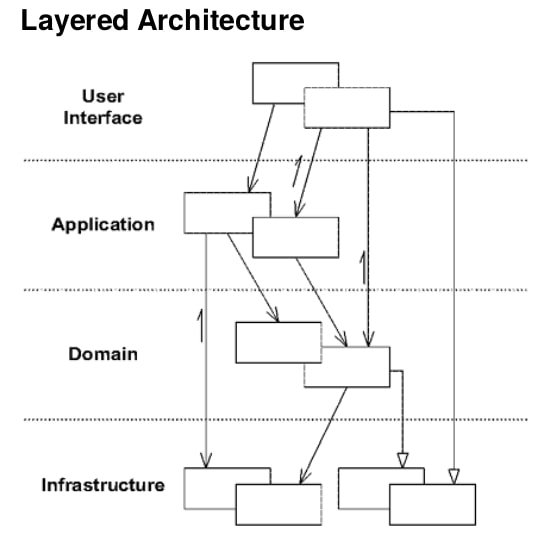
\includegraphics[width=0.5\textwidth]{docs/images/ch_2/DDD-Layered-Architecture-2.png} 
  \caption{Slojevi sistema \cite{dddfull}}
  \label{fig:sample}
\end{figure}

\section{Okruženje Nest.js}

NestJS \cite{nestjsdocs} je Node.js okruženje za razvoj serverskih aplikacija. Izgrađen je nad bibliotekom \textit{express} \cite{expressjsdocs} koja je i danas popularan izbor za izradu manjih serverskih aplikacija, kao i za edukativne svrhe. blabla još malo nalupam o Nest-u, mrzi me sad da čitam docs. U srž ovog okruženja ugrađeni su koncepti modula, servisa i umetanja zavistnosti (\textit{eng} Dependency Injection - u daljem tekstu \textbf{DI}), što ga čini idealnim za konstrukciju aplikacije zasnovane na DDD principima.

\section{Sloj infrastrukture}

Sloj infrastrukture ima više uloga u DDD sistemu, ali zajednička osobina je odsustvo iniciranja akcija u sloju domena \cite{dddfull}. Veliki deo ovog sloja često zauzima implementacija trajnosti podataka (\textit{eng. data persistence}), i to neretko šablonom repozitorijuma (\textit{eng. Repository pattern}). Uloga ovog šablona jeste odvajanje logike za čuvanje podataka van domenskog modela \cite{msrepository}. Često se ostvaruje uz pomoć jedne ili više klasa sa nekim uobičajenim metodama za dohvatanje ili ažuriranje entiteta.


\subsection{Repozitorijumi}
Apstrakcija koju pruža sloj repozitorijuma ogleda se upravo u načinu na koji on obrađuje podatke pre vraćanja u više slojeve, tačnije služi se \textbf{šablonom preslikavanja podataka} (\textit{eng Data mapper pattern} - stavi referencu). Uloga mapiranja podataka uglavnom je, u praksi, delegirana konkretnoj biblioteci ili okruženju koja upravlja pristupom bazi putem softverskog segmenta iz klase Objetno-relacionih ili Objektno-domenskih mapera (\textit{eng Object Relational Mapper - ORM, Object Document Mapper - ODM}). Iako ti sistemi često u potpunosti zadovoljavaju potrebe mapiranja podataka, u ovom radu je mapiranje urađeno manuelno, tako da se objekti dobijeni ODM slojem, odnosno bibliotekom \textit{mongoose - dodaj referency}, preslikavaju u entitete koristeći biblioteku \textit{@automapper/js, dodaj referencu}.

\begin{figure}[h]
  \centering
  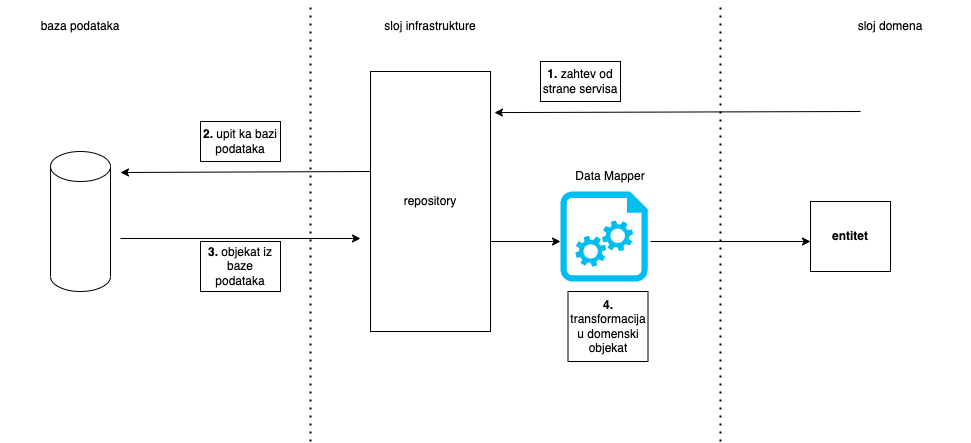
\includegraphics[width=1\textwidth]{docs/images/ch_2/repository.png} 
  \caption{Dijagram dohvatanja entiteta preko repozitorijuma}
  \label{fig:sample}
\end{figure}

Prirodno se nameće pitanje dohvatanja povezanih entiteta, ili konkretnije rad sa agregatima. U ovom radu implementiran je sistem \textbf{pohlepnog učitavanja} (\textit{eng Eager loading}), kojim se svi povezani entiteti zahtevanog entiteta dohvataju odmah prilikom zahteva ka glavnom entitetu. U nekim sistemima ovakav izbor ne bi bio idealan, međutim takva odluka je doneta u ovoj situaciji usled činjenice da je dizajn baze podataka relativno jednostavan, i lakoća implementacije i korišćenja nadmašuje cene u performansama, koje su minimalne. Kombinacija $populate$ metode biblioteke \textit{mongoose} i rekurzivne prirode biblioteke \textit{automapper/js} ovo se lako postiže.

U nastavku su primeri k\^{o}da iz repozitorijumske klase za pristup tiketima, odnosno glavnim entitetima datog sistema.

Na sledećem isečku vidimo zaglavlje klase \textit{TicketsRepository}. Kao i sve ostale repozitorijumske klase, oslanjaju se na model klase dobijene od strane biblioteke \textit{mongoose}, i deklarišu niz koji predstavlja sve putanje koje treba popuniti zarad implementacije pohlepnog učitavanja.

\begin{figure}[h]
\begin{lstlisting}[language=JavaScript, style=ES6, caption={Fajl \textit{tickets.repository.ts}, konstrukcija i niz POPULATE}]
export class TicketsRepository {
  constructor(
    @InjectModel(TicketDb.name) private ticketModel: Model<TicketDb>,
    @InjectMapper() private readonly mapper: Mapper,
  ) {}

  public static POPULATE = [
    {
      path: 'history.initiator',
      model: 'UserDb',
    },
    {
      path: 'history.payload.assignees',
      model: 'UserDb',
    },
    { path: 'createdBy', model: 'UserDb' },
    {
      path: 'tags',
      model: 'TicketTagDb',
      populate: { path: 'group', model: 'TicketTagGroupDb' },
    },
    { path: 'assignees', model: 'UserDb' },
    {
      path: 'history.payload.tags',
      model: 'TicketTagDb',
      populate: {
        path: 'group',
        model: 'TicketTagGroupDb',
      },
    },
  ];
\end{lstlisting}
\end{figure}

\newpage
Sledeći isečak prikazuje primer dohvatanja jednog tiketa putem identifikatora, pri čemu se, naravno, prilikom vraćanja rezultata vrši mapiranje u odgovarajući entitet.

\begin{figure}[h]
\begin{lstlisting}[language=JavaScript, style=ES6, caption={Fajl \textit{tickets.repository.ts}, dohvatanje entiteta}]
async findById(id: string): Promise<Ticket | null> {
    const result = await this.ticketModel
      .findById(id)
      .populate(TicketsRepository.POPULATE);
    
    if (!result) {
      return null;
    }
    
    return this.mapper.map(result, TicketDb, Ticket);
}
\end{lstlisting}
\end{figure}

\newpage
\subsection{Sheme i mutacije podataka, šablon Event Sourcing}
Osim repozitorijuma, sloj infrastrukture prirodno sadrži i definicije shema biblioteke \textit{mongoose}. Iz ugla programera, ovi objekti su najbliža pristupna tačka bazi podataka, i podržavaju operacije upita i mutacija nad realnim podacima u bazi. Takav jedan upit viđen je na isečku 2.4 u prethodnoj sekciji.

Na ovom mestu prikazujemo primer mutacije podataka, i to baš tiketa. Osim prikaza rada sa mutiranjem podacima kroz biblioteku \textit{mongoose}, ovaj primer služi da ilustruje dualnu prirodu tiketa kao entiteta, i njegovu potpunu različitost u strukturi između sloja infrastruktura i sloja domena. Naime, kao što će biti prikazano u sledećem poglavlju, tiket u sloju domena je jednostavna klasa koja sadrži sve podatke o datom tiketu. Ipak, u sloju infrastrukture, radi veće fleksibilnosti i mogućnosti praćenja istorije, upotrebljena je varijanta šablona \textit{Event Sourcing}. Osnovno načelo ovog šablona je da umesto čuvanja eksplicitnog stanja objekta čuvamo istoriju njegovih promena.
Ovde cu da pokazem ukratko kako se tiket mutira, kako dodajemo u istoriju stvari, i kako se to persistuje i pri mapiranju vraca u sloj domena, jako me mrzi to sad da radim pa ostavljam za posle


\newpage
\section{Sloj domena}

Takođe poznat kao srce poslovnog softvera, sloj domena sadrži glavnu poslovnu logiku i operacije koje direktno oslikavaju dešavanja u svetu koji softver module. Iz ugla implementacije, svoje mogućnosti pružaju putem apstrakcije koju često nazivamo servisima, što koristimo i kao sufiks u nazivima njihovih klasa, iako se mogu koristiti i druge konvencije\footnote{Nekad se umesto sufiksa \textit{Service} koriste reči koje direktno oslikavaju namenu datog servisa. Na primer umesto \textit{GetUserService} koristi se naziv \textit{UserProvider} i sl.}.

% ------------------------------------------------------------------------------
\chapter{Frontend}
\section{Okruženje Next.js, serversko renderovanje React komponenti}
\section{Upravljanje stanjem aplikacije}
\section{Internacionalizacija}

% ------------------------------------------------------------------------------

% ------------------------------------------------------------------------------
\chapter{Analitika}
\section{Skladišta podataka, ETL procesi}
\section{Prikaz metrika, biblioteka Streamlit}
% ------------------------------------------------------------------------------

% ------------------------------------------------------------------------------
\chapter{Devops}
\section{Virtuelizacija, sistem Docker}
\section{nginx kao reverzni proksi}
% ------------------------------------------------------------------------------

% ------------------------------------------------------------------------------
\chapter{Zakljucak}
% ------------------------------------------------------------------------------
% ------------------------------------------------------------------------------
% Literatura
% ------------------------------------------------------------------------------
\literatura

% ==============================================================================
% Završni deo teze i prilozi
\backmatter
% ==============================================================================

% ------------------------------------------------------------------------------
% Biografija kandidata
\begin{biografija}
Lako ćemo to
\end{biografija}
% ------------------------------------------------------------------------------

\end{document} 
